\chapter{Architecture} \label{chapter5}

    The architecture of this project is developed using an Object Oriented Programming (\acrshort{oop}) approach such that each data type and its associated methods are kept in separate classes. Furthermore, this application actively uses concepts involving data encapsulation and abstraction, inheritance, polymorphism, and dynamic binding.

\section{Mobile technology} \label{5:mobile_technology}

    Smartphones have become indispensable to human life, especially since they began to replace the need for additional gadgets, besides the leading role of calling people.
    
    As a result, we opted to implement a mobile solution for students. We offer a painless and favorable user experience on a device not missing from the pocket of anyone. Thus, students can find various information or conveniently perform multiple tasks and actions in a time-saving manner.
    
    \textbf{Flutter}\footnote{https://flutter.dev/} represents a cross-platform toolkit developed by Google that allows the development of attractive designs without significant effort, given the multitude of already predefined \acrshort{ui} components, called \textit{widgets}.
    
    As technology, Flutter uses \textbf{Dart}\footnote{https://dart.dev/}, a client-optimized solution that allows great development flexibility, null safety features, built-in collections, and support for asynchronous methods. Equally, this technology grants fast incremental compilation for applications targeting mobile and desktop devices, as well as the web environment.

\section{Database} \label{5:database}

    To benefit from a database with real-time information updates, built-in security mechanisms, and cloud storage convenience, we continued using the services offered by \textbf{Firebase}\footnote{https://firebase.google.com/}, as described in \textit{Design and Implementation of a Cross-Platform Mobile Application That Facilitates Student Collaboration} \cite{ioana2020paper}.
    
    \subsection{Firestore} \label{5:firestore}
    
    \textbf{Cloud Firestore} represents a \textit{No\acrshort{sql}} type database designed for both mobile and web development applications. With its help, data can be stored in different collections. In its turn, a collection is made up of multiple documents, and each document can contain from elementary strings, booleans, and numbers, to complex, nested objects in addition to subcollections. At the same time, it is not mandatory that all the documents located in a collection have the same fields, but on the contrary, they may differ.
    
    As a result, we can confirm that Firestore offers a substantial degree of flexibility to an application by maintaining a dynamic architecture for unstructured data. Furthermore, it provides the ability to handle a large volume of requests from users simultaneously, and it is not dependent on a permanent connection to the Internet. Thus, Firestore has the advantage of providing support for offline actions by caching actively used data. Eventually, any offline modifications performed will be synchronized again when the online connection is restored.
    
    \subsection{Database structure used} \label{5:database_structure}
    
    To manage all the references about users, people, questions, and answers of the feedback form, our application uses several separate collections. Therefore, we can administer and systematically handle all the details stored efficiently.
    
    As our project benefits from a flexible structure, we consider the possibility of specific fields from a document to have a null value, especially if a student does not want to answer a particular question. However, to reduce the total number of \textit{read} and \textit{write} operations (fig. \ref{5:fig:firestore_operations}) and the size of the database, we decided not to store any empty information.
    
    \begin{figure}[!ht]
        \centering
         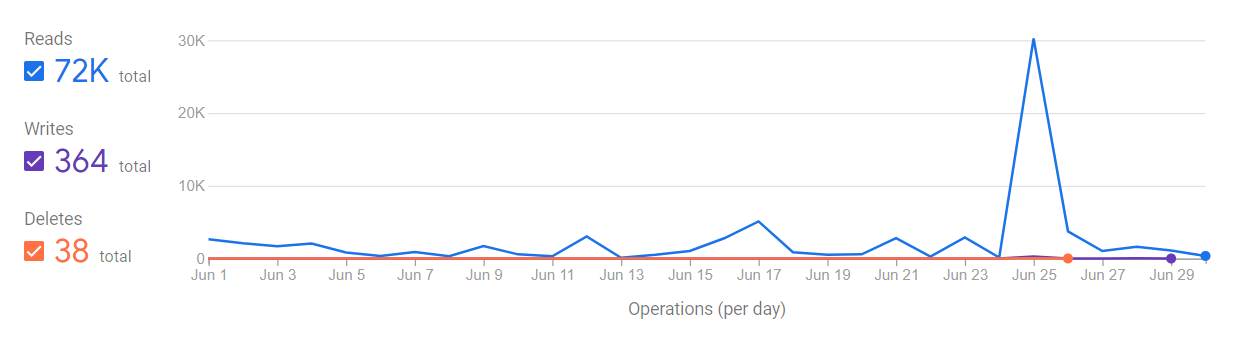
\includegraphics[width=1\textwidth]{figures/charts/firestore_operations.png}
         \caption{Number of operations for our application, as reported by Firestore, in the last 30 days}
        \label{5:fig:firestore_operations}
    \end{figure}

    We will further present the collections used in this application from the point of view of all the data that represents the subject of this thesis.
    
    ~
    
    \faDatabase \hspace{0.1cm} \textbf{\mintinline{text}{users}}
    
    This collection permits storing data about the classes of a student, together with a list mentioning all the subjects where the feedback questionnaire was already completed. This information is required as not to complete the feedback form for a specific class more than once.
    
    \begin{table}[th]\small\linespread{1}
        \centering
        \caption{\textbf{users} collection additions}
        \label{5:tab:users}
        \begin{tabular}{| l | l | c | p{4.7cm} |}
        \hline
        \textbf{Field} & \textbf{Type} & \textbf{Required?} & \textbf{Additional info} \\
        \hline
        classes & \mintinline{text}{array<string>} & \Checkedbox & list of classes in which the user is enrolled 
        \\
        \hline
        classesFeedback & \mintinline{text}{map<string, boolean>} & \CrossedBox & specifies whether the user completed or not the feedback form for a class
        \\
        \hline
        \end{tabular}
    \end{table}
    
    \clearpage
    
    \faDatabase \hspace{0.1cm} \textbf{\mintinline{text}{people}}

    This collection has been defined since the first version of the application \cite{ioana2020paper}. It contains details that reference the name, email address, photo, and position of a teacher, along with their office location. However, we have also added information related to the department of a teacher, along with their phone number. Each field in this collection is a \textit{string}, including their picture, represented as a \acrshort{url}.
    
    \faDatabase \hspace{0.1cm} \textbf{\mintinline{text}{forms}}
    
    This collection represents the primary source of information for the functionalities described. Initially, its purpose was to collect requests from users to change their permission level to contribute with various details introduced in the application, such as events in the timetable or information about a particular class, like grading, valuable links, and resources. This form can be accessed by each user from the \textit{Settings} page of the application.
    
    \begin{table}[th]\small\linespread{1}
        \centering
        \caption{\textbf{forms} collection structure}
        \label{5:tab:forms}
        \begin{tabular}{| l | l | c | p{4.7cm} |}
        \hline
        \textbf{Field} & \textbf{Type} & \textbf{Required?} & \textbf{Additional info} \\
        \hline
        addedBy & \mintinline{text}{string} & \CrossedBox & the ID of the user who submitted the request
        \\
        \hline
        dataSubmitted & \mintinline{text}{timestamp} & \CrossedBox & field   that records the timestamp when a request was sent
        \\
        \hline
        requestBody & \mintinline{text}{string} & \Checkedbox & actual message sent by a user
        \\
        \hline
        \end{tabular}
    \end{table}
    
    Subsequently, to benefit from a database architecture as compact as possible, we decided to introduce two other documents in the same collection.
    
    The first document is responsible for storing all the questions from the feedback questionnaire and their corresponding categories. The structure of this document is presented in table \ref{5:tab:class-feedback-questions}. In addition, we outline the format of a question in table \ref{5:tab:feedback-question}.
    
    The second document has a more complex structure. It is composed of multiple subcollections, whose keys are defined by the number of the question in the feedback form. Furthermore, each subcollection consists of a list of documents with an automatically generated key, while each document represents the answer submitted by a user to that question. As we reach the end of the hierarchy, an answer is composed of the actual value (the result or the comment provided), together with the details related to a class (its name, associated teacher, and assistant). To provide anonymity, we do not retain the ID of the user who completed a questionnaire. The structure of this data set is highlighted in table \ref{5:tab:class-feedback-answers}.
    
    \begin{table}[th]\small\linespread{1}
        \centering
        \caption{\textbf{class\_feedback\_questions} document structure}
        \label{5:tab:class-feedback-questions}
        \begin{tabular}{| l | p{2.6cm} | c | p{7.1cm} |}
        \hline
        \textbf{Field} & \textbf{Type} & \textbf{Required?} & \textbf{Additional info} \\
        \hline
        categories & \mintinline{text}{map<string,}
        
        \mintinline{text}{ map<string,}
        
        \mintinline{text}{ string>>} & \CrossedBox & nested map composed of the category name as key and another map as value, which stores pairs of elements that contain the language reference and the corresponding localized category name
        \\
        \hline
        questions & \mintinline{text}{map<string,}
        \mintinline{text}{ feedback_}
        \mintinline{text}{question>} & \CrossedBox & the data structure which stores all the questions from the feedback form
        \\
        \hline
        \end{tabular}
    \end{table}
    
    \begin{table}[th]\small\linespread{1}
        \centering
        \caption{\textbf{feedback\_question} type structure}
        \label{5:tab:feedback-question}
        \begin{tabular}{| l | p{2.6cm} | c | p{7.1cm} |}
        \hline
        \textbf{Field} & \textbf{Type} & \textbf{Required?} & \textbf{Additional info} \\
        \hline
        category & \mintinline{text}{string} & \CrossedBox & category name; the value of this field corresponds to the key of the nested map \textit{categories} from \textbf{class\_feedback\_questions} document
        \\
        \hline
        question & \mintinline{text}{map<string,}
        \mintinline{text}{string>} & \CrossedBox & stores the actual question as value, while the key specifies the language ("en", "ro")
        \\
        \hline
        type & \mintinline{text}{string} & \CrossedBox & one of: "rating", "dropdown", "text", "slider"
        \\
        \hline
        options & \mintinline{text}{array<}
        \mintinline{text}{map<string,}
        \mintinline{text}{string>>} & \CrossedBox & answer options for dropdown questions; key of the map contains the language, whereas the value corresponds to the localized answer
        \\
        \hline
        \end{tabular}
    \end{table}
    
    \clearpage
    
    \begin{table}[th]\small\linespread{1}
        \centering
        \caption{\textbf{class\_feedback\_answers} collection structure}
        \label{5:tab:class-feedback-answers}
        \begin{tabular}{| l | l | c | p{4.7cm} |}
        \hline
        \textbf{Field} & \textbf{Type} & \textbf{Required?} & \textbf{Additional info} \\
        \hline
        answer & \mintinline{text}{string} & \HollowBox & actual value of the answer provided for a question 
        \\
        \hline
        assistant & \mintinline{text}{string} & \Checkedbox & name of the assistant
        \\
        \hline
        class & \mintinline{text}{string} & \CrossedBox & id of the class for which feedback is given
        \\
        \hline
        dateSubmitted & \mintinline{text}{timestamp} & \CrossedBox & the field that records the exact time when the feedback form was sent
        \\
        \hline
        teacher & \mintinline{text}{string} & \Checkedbox & name of the teacher
        \\
        \hline
        \end{tabular}
    \end{table}
    
    \subsection{Remote Config} \label{5:remote_config}
    
    \textbf{Remote Config}\footnote{https://firebase.google.com/docs/remote-config} is a service provided by the Firebase platform, which can make changes in our application without republishing it.
    
    In our case, we propose a solution that offers students the ability to provide feedback only within a well-established time frame. Thus, although our functionalities will everlastingly be integrated with the application, these will not always be accessible by our users.
    
    To initialize this option, we defined a parameter (fig. \ref{5:fig:feedback_enabled}) based on which features we offer are hidden or not. It contains a default value and the condition (fig. \ref{5:fig:feedback_option}) that can modify it.
    
    \begin{figure}[!ht]
        \centering
         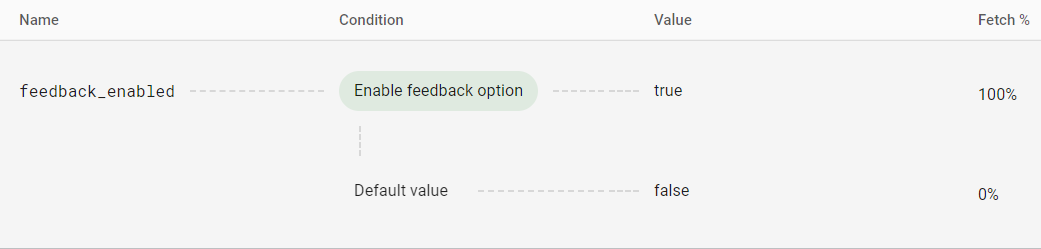
\includegraphics[width=1\textwidth]{figures/feedback_enabled.png}
         \caption{Remote Config parameter values, as shown in the Firebase interface}
        \label{5:fig:feedback_enabled}
    \end{figure}
    
    \clearpage
    
    \begin{figure}[!ht]
        \centering
         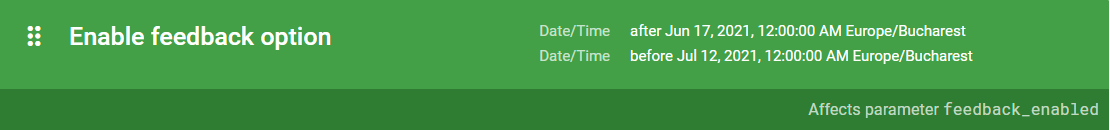
\includegraphics[width=1\textwidth]{figures/feedback_option.png}
         \caption{Condition used to enable feedback, as displayed by Firebase}
        \label{5:fig:feedback_option}
    \end{figure}
    
    We implemented the Remote Config option using the \textbf{Singleton} design pattern to restrict its instantiations to a single object. Moreover, we define a map that stores a default value that needs to be used if the application cannot fetch the configuration parameter from the database.

\section{System implementation} \label{5:system_implementation}

    The contribution\footnote{https://github.com/student-hub/acs-upb-mobile/blob/master/CONTRIBUTING.md} to this project respects a strict policy of code writing so that the structure of the application is modular and easy to understand. Moreover, boilerplate code sections are almost non-existent since we are constantly looking to reuse already developed components.

\subsection{Development process} \label{5:development_process}

    To obtain a satisfactory final result, the whole mechanism we use for development is quite complex, and it follows a well-established code of conduct\footnote{https://github.com/student-hub/acs-upb-mobile/blob/master/CODE\_OF\_CONDUCT.md}.
    
    Firstly, the act of planning and analyzing plays a crucial role in order to create valid and reliable solutions. All our decisions are implemented after consultation with the entire project team.
    
    We use \textit{git\footnote{https://git-scm.com/}} as a way to version the code and \textbf{GitHub} as a hosting service. Therefore, each developer needs to work on his branch. Each contributor has to submit a new Pull Request (\acrshort{pr}) to maintain visibility on the implementation. Our contribution can be merged into the production environment after a serious review process. In addition, each \acrshort{pr} needs at least one approval from a team member.
    
    To remove error-prone situations, our project uses two different databases for both production and development environments. In this way, we ensure our users that their data is not accidentally altered or modified.
    
    Overall, although the policy of our system is based on a relatively slow-moving advancement, it allows us to offer users a well-defined and error-free ecosystem.

\subsection{Project structure} \label{5:project_structure}

    This project uses the \textbf{\acrshort{bloc}} (Business Logic Component) design pattern, slightly modified by separating the \acrshort{ui} modules from the actual data layer and providing a state management system, in combination with the use of provider modules. The entire logic of this configuration is focused on accepting and processing events, based on which the state of any page in the application can change.
    
    \begin{wrapfigure}{r}{0.35\columnwidth}
            \centering
            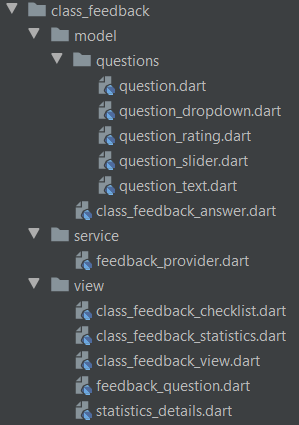
\includegraphics[width=0.4\columnwidth]{figures/project_structure.png}
            \captionsetup{labelsep=space, textformat=empty}
            \caption{The hierarchy of files and folders from our project structure}
            \label{5:fig:project_structure}
    \end{wrapfigure}
    
    To respect the database structure described in section \ref{5:database_structure}, we organized our setup in multiple packages (an example is illustrated in fig. \ref{5:fig:project_structure}), depending on their role:
    
    \begin{itemize}
            \setlength{\topsep}{0.5pt}
            \setlength{\itemsep}{0.5pt}
            \setlength{\parsep}{0.5pt}
            \item \textbf{model}: represents the data level of the application
            \item \textbf{service}: contains all the providers that interact directly with our database; according to the developers\footnote{https://pub.dev/packages/provider} of this concept, a provider has the role in \textit{creating, listening, or dispose} of the information; each provider module defined has precise methods by which data is extracted or added
            \item \textbf{view}: represents the presentation level of the application; it displays the model information to each user
\end{itemize}

\section{Testing} \label{5:testing}

    Being an application that benefits from continuous development from our team, each student working on its task, testing our features becomes mandatory.
    
    Although we could consider, at first sight, that everything works nominally following some code changes in our application, it has been proven that we might wake up with unpleasant surprises any time, even at the slightest adjustments.
    
    Our team relied on manual and automatic testing throughout the various functionalities implemented, verifying our code additions rigorously.
    
    Since our project consists of a cross-platform solution and considering the multitude of gadgets available on the current market, our initial step in developing the test modules was to define several screen resolutions, for instance, 720x1280 or 600x1024 pixels. Therefore, we can ensure that \acrshort{ui} elements are displayed properly, regardless of the device used.
    
    Moreover, regarding packages used, our application adopted the \textbf{\textit{flutter\_test}}\footnote{https://api.flutter.dev/flutter/flutter\_test/flutter\_test-library.html} library, which allows the verification of each \acrshort{ui} component, including different page navigation and buttons pressing simulation. According to \textit{Codecov}\footnote{https://about.codecov.io/}, our complete set of features is currently being tested in a proportion of approximately \textbf{68\%}. In addition, the evolution over time can be observed in figure \ref{5:fig:codecov}:
    
    \begin{figure}[!ht]
        \centering
         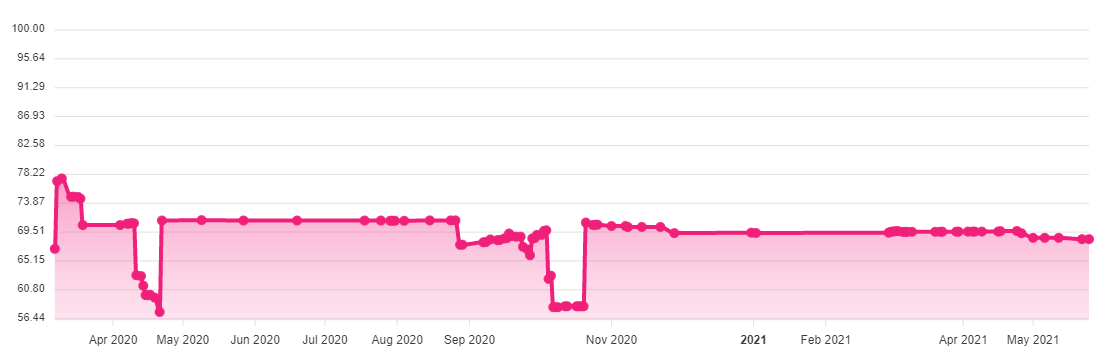
\includegraphics[width=0.95\textwidth]{figures/charts/codecov.png}
         \caption{Code coverage evolution}
        \label{5:fig:codecov}
    \end{figure}
    
    However, the difference up to 100\% is caused by the lack of testing for the provider modules interacting with Firestore. Thus, we had to mock our database directly in the test files, including the results of all asynchronous calls used in communication with every Firebase section. As a result, we frequently had to deal with flaky tests, so we are thinking about refactoring all testing processes using \textbf{\textit{flutter\_driver}}\footnote{https://api.flutter.dev/flutter/flutter\_driver/flutter\_driver-library.html} dependency.
    
    